\emph{
    Ejecute y explique la funci\'on del siguiente c\'odigo en Octave. 
    Incluya una gr\'afica en la que la longitud de la variable k sea mayor a 1000. 
    (Puede modificar el programa...) En la gr\'afica observara un esbozo de la 
    trayectoria de un proceso de ramificaci\'on continuo (en una escala distinta...).
    \texttt{
        \lstinputlisting[caption=]{tarea3/problema3_4/binaryGW.R}
    }
}

\afterstatement\pn

El código simula un proceso de Galton-Watson.\pn

\texttt{k = [10]} significa que al inicio habrá 10 individuos.\pn

\texttt{aux} es la última población obtenida. \texttt{binornd(aux, .5)} es una instrucción de Octave en la que
de un conjunto de \texttt{aux} elementos, escoge a cada uno con probabilidad \texttt{.5}. El resultado
es el número de elementos seleccionados. Multiplicar esto por \texttt{2} se puede interpretar como que
antes de morir, cada individuo seleccionado tiene dos hijos.\pn

\texttt{k = [k; 2*binornd(aux, .5)]} está agregando al vector \texttt{k} una nueva entrada. La entrada,
es la nueva población, resultante de que cada individuo seleccionado tiene dos hijos antes de morir y cada
elemento no seleccionado muere sin tener decendientes.\pn
 
A continuación, una gráfica con una ejecución de este algoritmo comenzando con \texttt{10} individuos
y terminando con \texttt{0} individuos después de un poco más de \texttt{12000} iteraciones.

\begin{center}
    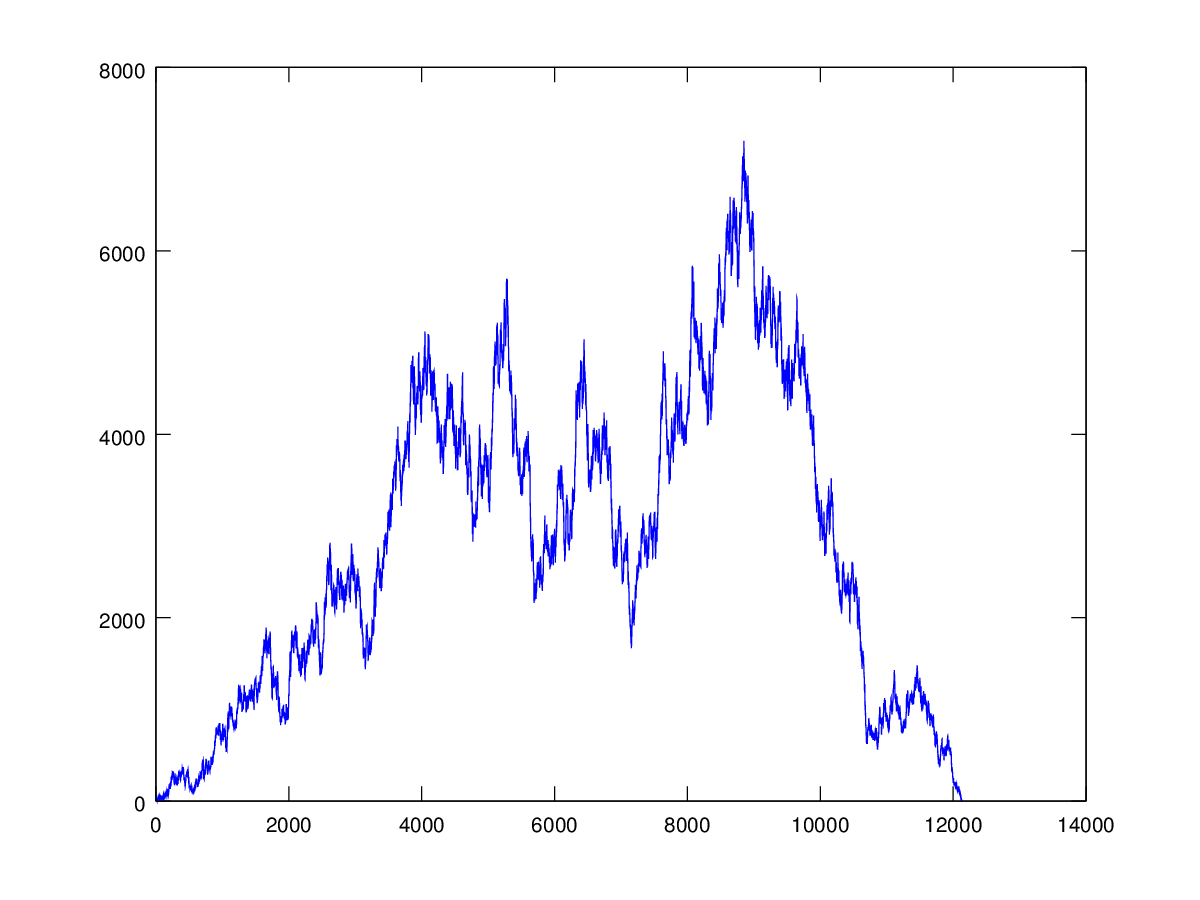
\includegraphics[width=8cm]{tarea3/problema3_4/galtonWatson.PNG}
    
    Gr\'afica de una ejecuci\'on del proceso de extinci\'on de Galton-Watson 
    Par\'ametros:\par
    10 individuos\par 
    La probabilidad de que un individuo tenga $2$ hijos es $\frac{1}{2}$\par
    La probabilidad de que un individuo tenga $0$ hijos es $\frac{1}{2}$.\pn
\end{center}

La esperanza de número de decendientes que tiene un individuo, es \texttt{1}. Es decir,
este proceso de Galton-Watson es crítico. En clase se demostró que los procesos Galton-Watson
críticos se extinguen con probabilidad \texttt{1}. La gráfica arriba mostrada es de una corrida
del algoritmo que más iteraciones duró antes de extinguirse, el algoritmo, se corrió
\texttt{200,000} veces y, en todos los casos se extingió la población. Esto es consistente con
con el resultado teórico (en todos los casos, de un conjunto de \texttt{200,000}, la población se extinguió).\pn

A continuación, una gráfica resultante del mismo algoritmo, pero con una población inicial de \texttt{1000} individuos.
que se extingue después de \texttt{20,000} iteraciones. Cabe mencionar que esta corrida fue más ``suertuda'' que la
representada en la gráfica anterior. Muchas de las corridas del algoritmo sin modificar superaron una población de
\texttt{1000} individuos en algún momento y después de eso, nunca duraron tanto como este otro.

\begin{center}
    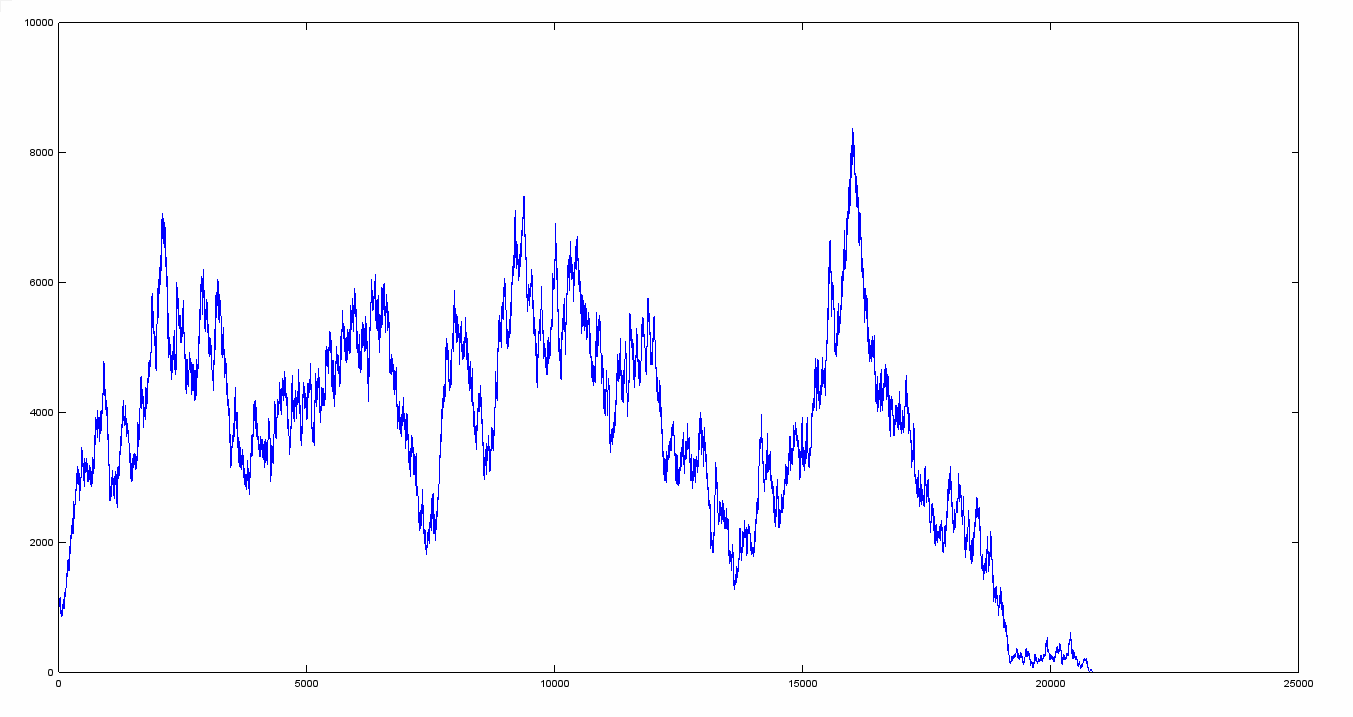
\includegraphics[width=12cm]{tarea3/problema3_4/galtonWatsonEmpezandoEn1000.PNG}
    
    Gr\'afica de una ejecuci\'on del proceso de extinci\'on de Galton-Watson 
    Par\'ametros:\par 
    1000 individuos iniciales \par
    La probabilidad de que un individuo tenga $2$ hijos es $\frac{1}{2}$ \par
    La probabilidad de que un individuo tenga $0$ hijos es $\frac{1}{2}$.\pn
\end{center}

P.S. El algoritmo modificado se incluye bajo el nombre de \par
\texttt{BinaryGWModificado.R}. (Incluí un candado para que el algoritmo terminara si 
superaba un millón de iteraciones, nunca se alcanzó dicho límite).